% Copyright 2004 by Till Tantau <tantau@users.sourceforge.net>.
%
% In principle, this file can be redistributed and/or modified under
% the terms of the GNU Public License, version 2.
%
% However, this file is supposed to be a template to be modified
% for your own needs. For this reason, if you use this file as a
% template and not specifically distribute it as part of a another
% package/program, I grant the extra permission to freely copy and
% modify this file as you see fit and even to delete this copyright\usecolortheme[named=CornellRed]{structure}
% notice. 

\documentclass[xcolor = dvipsnames]{beamer}
%\usefonttheme{serif}
\usepackage{graphicx, caption}

\usepackage{subcaption}
\usepackage{amsmath,amscd, amsthm, mathrsfs, amssymb, esint}
\usepackage{graphics}
\usepackage{mathtools}
\usepackage{biblatex}

\useoutertheme{miniframes} % Alternatively: miniframes, infolines, split
\useinnertheme{circles}

\definecolor{CornellRed}{RGB}{179, 27, 27} % UBC Blue (primary)

\usecolortheme[named=CornellRed]{structure}
% There are many different themes available for Beamer. A comprehensive
% list with examples is given here:
% http://deic.uab.es/~iblanes/beamer_gallery/index_by_theme.html
% You can uncomment the themes below if you would like to use a different
% one:
%\usetheme{AnnArbor}
%\usetheme{Antibes}
%\usetheme{Bergen}
%\usetheme{Berkeley}
%\usetheme{Berlin}
%\usetheme{Boadilla}
%\usetheme{boxes}
%\usetheme{CambridgeUS}
%\usetheme{Copenhagen}
%\usetheme{Darmstadt}
%\usetheme{default}
%\usetheme{Frankfurt}
%\usetheme{Goettingen}
%\usetheme{Hannover}
%\usetheme{Ilmenau}
%\usetheme{JuanLesPins}
%\usetheme{Luebeck}
%\usetheme{Madrid}
%\usetheme{Malmoe}
%\usetheme{Marburg}
%\usetheme{Montpellier}
%\usetheme{PaloAlto}
%\usetheme{Pittsburgh}
\usetheme{Rochester}
%\usetheme{Singapore}
%\usetheme{Szeged}
%\usetheme{Warsaw}
\usepackage{amsmath,amscd, amsthm, mathrsfs, amssymb, esint}
\usepackage{graphicx}
\usepackage{float}

\usepackage{subcaption}
%\usepackage{subfig}
\usepackage{mathtools}
%\DeclarePairedDelimiter\abs{\lvert}{\rvert}


\makeatother
\usepackage{array}
\usepackage{booktabs}

\newcommand{\lap}{\Delta}





\setbeamersize{text margin left=5mm,text margin right=5mm} 
\title{Analysis on Fractals: Sobolev Orthogonal Polynomials on the Sierpinski Gasket}

% A subtitle is optional and this may be deleted


\author{Max Jiang, Tian Lan, Shashank Sule, Sreeram Venkat, Xiaoduo Wang\\[0.4cm]Advisors: Kasso Okoudjou and Robert Strichartz}
% - Give the names in the same order as the appear in the paper.
% - Use the \inst{?} command only if the authors have different
%   affiliation.

\institute{Cornell SPUR 2019: Analysis on Fractals}% (optional, but mostly needed)

% - Use the \inst command only if there are several affiliations.
% - Keep it simple, no one is interested in your street address.

\date{\today}
% - Either use conference name or its abbreviation.
% - Not really informative to the audience, more for people (including
%   yourself) who are reading the slides online

%\subject{MATH 320}
% This is only inserted into the PDF information catalog. Can be left
% out. 

% If you have a file called "university-logo-filename.xxx", where xxx
% is a graphic format that can be processed by latex or pdflatex,
% resp., then you can add a logo as follows:

% \pgfdeclareimage[height=0.5cm]{university-logo}{university-logo-filename}
% \logo{\pgfuseimage{university-logo}}

% Delete this, if you do not want the table of contents to pop up at
% the beginning of each subsection:

\AtBeginSubsection[]
{
  \begin{frame}<beamer>{Outline}
    \tableofcontents[currentsection,currentsubsection]
  \end{frame}
}

% Let's get started
\begin{document}

\begin{frame}
  \titlepage
\end{frame}

\begin{section}{Introduction}

\begin{frame}{The Sierpinski Gasket}
    \begin{figure}
        \centering
        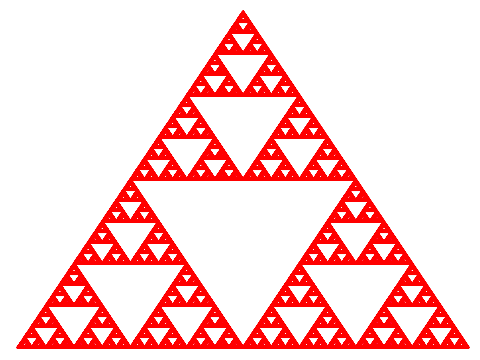
\includegraphics[width=0.45\linewidth]{Final_presentation/images/SG.png}
        \caption{The Sierpinski Gasket}
        %\label{fig:V0}
    \end{figure}
    
    Let $V_0 = \{q_0, q_1, q_2\} \in \mathbb{R}^2$ and $F_i(x) = \frac{1}{2}(x+q_i)$ for $i=0,1,2$. Then $$SG = \overline{\bigcup_{m=1}^{\infty}\bigcup_{|w|=m}F_w(V_0)}$$
    
\end{frame}
\begin{frame}{The Sierpinski Gasket}
    We work on the finite graph approximation $V_m = \bigcup_{|w|=m}F_{w}(V_0)$
    \begin{figure}
        \centering
        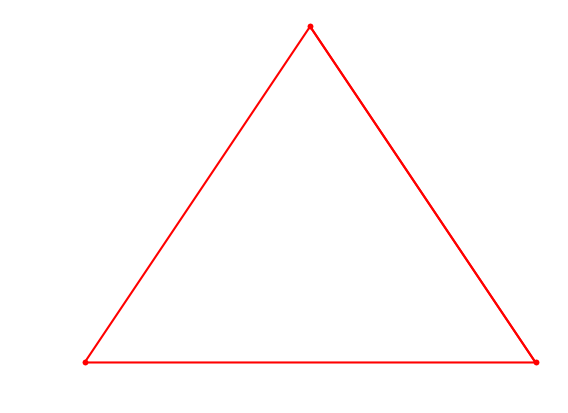
\includegraphics[width=0.7\linewidth]{images/V0.png}
        \caption{$V_0$}
        %\label{fig:V0}
    \end{figure}
\end{frame}
\begin{frame}{The Sierpinski Gasket}
    We work on the finite graph approximation $V_m = \bigcup_{|w|=m}F_{w}(V_0)$
    \begin{figure}
        \centering
        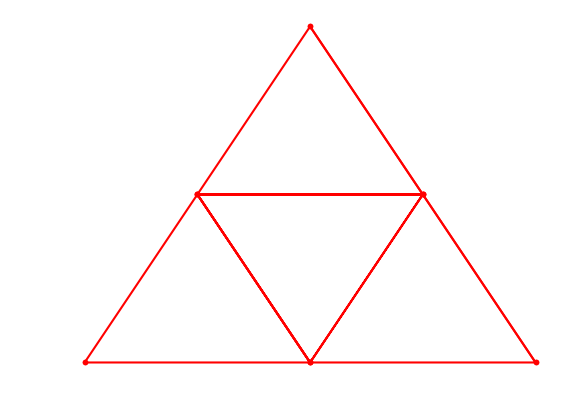
\includegraphics[width=0.7\linewidth]{images/V1.png}
        \caption{$V_1$}
        %\label{fig:V1}
    \end{figure}
\end{frame}

\begin{frame}{The Sierpinski Gasket}
    We work on the finite graph approximation $V_m = \bigcup_{|w|=m}F_{w}(V_0)$
    \begin{figure}
        \centering
        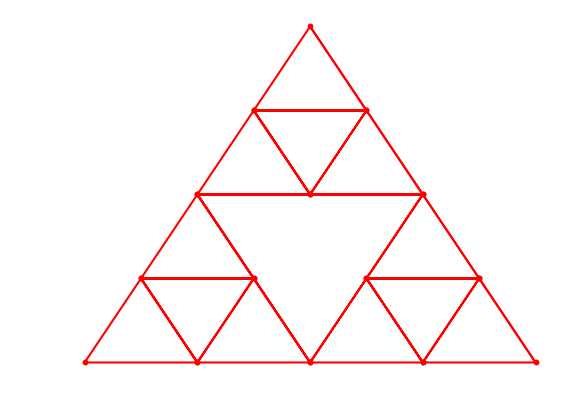
\includegraphics[width=0.7\linewidth]{images/V2.png}
        \caption{$V_2$}
        %\label{fig:V2}
    \end{figure}
\end{frame}

\begin{frame}{The Sierpinski Gasket}
    We work on the finite graph approximation $V_m = \bigcup_{|w|=m}F_{w}(V_0)$
    \begin{figure}
        \centering
        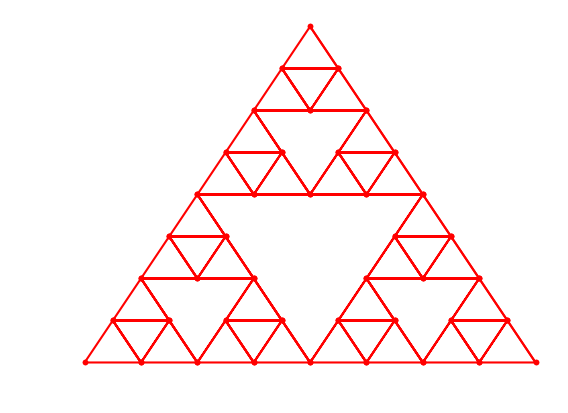
\includegraphics[width=0.7\linewidth]{images/V3.png}
        \caption{$V_3$}
        %\label{fig:V3}
    \end{figure}
\end{frame}

\begin{frame}{The Sierpinski Gasket}
    We work on the finite graph approximation $V_m = \bigcup_{|w|=m}F_{w}(V_0)$
    \begin{figure}
        \centering
        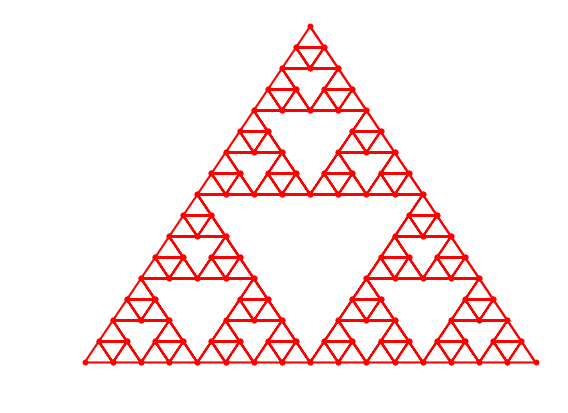
\includegraphics[width=0.7\linewidth]{images/V4.png}
        \caption{$V_4$}
        %\label{fig:V4}
    \end{figure}
    \pause
Note that $V_{*} = \bigcup_{m \in \mathbb{N}}V_m \neq SG$. However, $V_{*}$ is a dense and countable subset. 
\end{frame}


\begin{frame}{Calculus on the Sierpinski Gasket}
    \begin{itemize}
        \item Let $C = F_w(SG)$ denote an $m$ cell where $F_w = F_{i_m}\ldots F_{i_1}$. Then the \textbf{self similar measure} $\mu$ assigns weight $1/3^m$ to $C$. The self-similar measure $\mu$ is a regular Borel probability measure. 
        \pause
        \item Let $u: SG \mapsto \mathbb{R}$. Then the \textbf{Laplacian} $\Delta_{\mu}$ is defined as
        $$  \Delta_{\mu}u(x) = \frac{3}{2}\lim_{m \to \infty}5^m\Delta_mu(x)$$
        where $\Delta_mu(x) = \sum_{y \underset{m}{\sim} x}(u(x) - u(y))$
    \end{itemize}
\end{frame}
\begin{frame}{Calculus on the Sierpinski Gasket}
    \begin{itemize}
        \item $G: SG \times SG \mapsto \mathbb{R}$ is called \textbf{Green's Function} where
        $$ -\Delta u = f, u|_{V_0} = 0 \iff u(x) = \int_{SG}G(x,y)f(y)\,d\mu$$
        \pause
        \item $\partial_nu(q_i)$ is the \textbf{normal derivative} of $u$ at $q_i$ where
        $$ \partial_nu(q_i) = \lim_{m \to \infty}\Big(\frac{5}{3}\Big)^m(2u(q_i) - u(F^{m}_{i+1}q_i) - u(F^{m}_{i-1}q_i))$$
        \pause
        \item $\partial_Tu(q_i)$ is the \textbf{tangential derivative} of $u$ at $q_i$ where
        $$ \partial_{T}u(q_i) = \lim_{m\to\infty}5^m(u(F^{m}_{i+1}q_i) - u(F^{m}_{i-1}q_i))$$
    \end{itemize}
\end{frame}
\end{section}
\begin{section}{Polynomials on the Sierpinski Gasket}
\begin{frame}{Polynomials on SG}
    \begin{itemize}
        \item Let $f: SG \mapsto \mathbb{R}$. Then $f$ is a $j$-degree polynomial iff\\
        $\Delta^{j+1}f = 0$ and $\Delta^{j}f\neq 0$, i.e $f$ is $j$-harmonic but not ($j-1$)-harmonic. 
        \pause
        \item The space of polynomials with degree $\le j$ is denoted $\mathcal{H}_{j}$
        \pause
        \item We introduce the following basis $\{P_{jk}\}$ where
        \begin{align*}
            \Delta^nP_{jk}(q_0) &= \delta_{nj}\delta_{k1}\\
            \Delta^n\partial_nP_{jk}(q_0) &= \delta_{nj}\delta_{k2}\\
            \Delta^n\partial_TP_{jk}(q_0) &= \delta_{nj}\delta_{k3}\\
        \end{align*}
        This is known as the \textbf{monomial basis}
        \end{itemize}
\end{frame}

\begin{frame}{Polynomials on SG: The monomial basis}
    \begin{figure}[H]
        \centering
        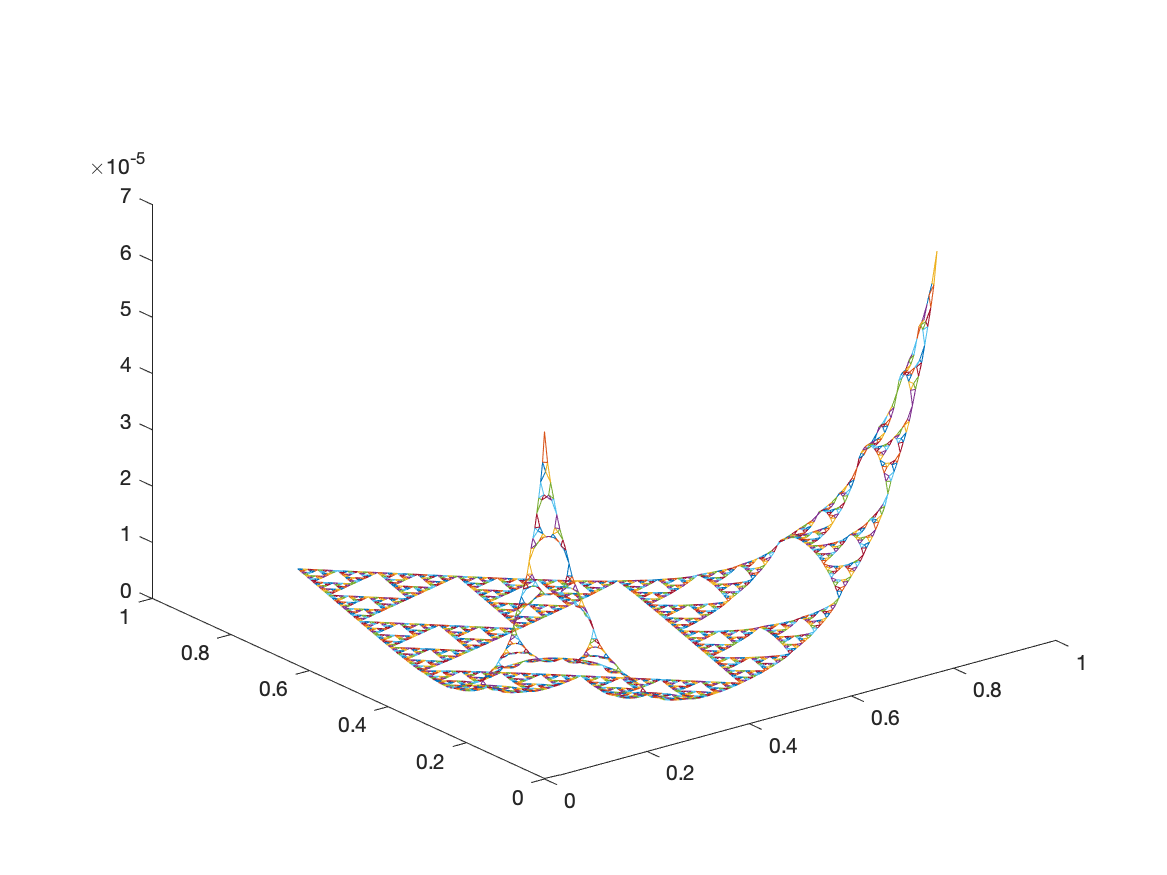
\includegraphics[width=0.75\linewidth]{Final_presentation/monomial3_1.png}
        \caption{$P_{31}$}
    \end{figure}
\end{frame}

\begin{frame}{Polynomials on SG: The monomial basis}

    \begin{figure}[H]
        \centering
        
        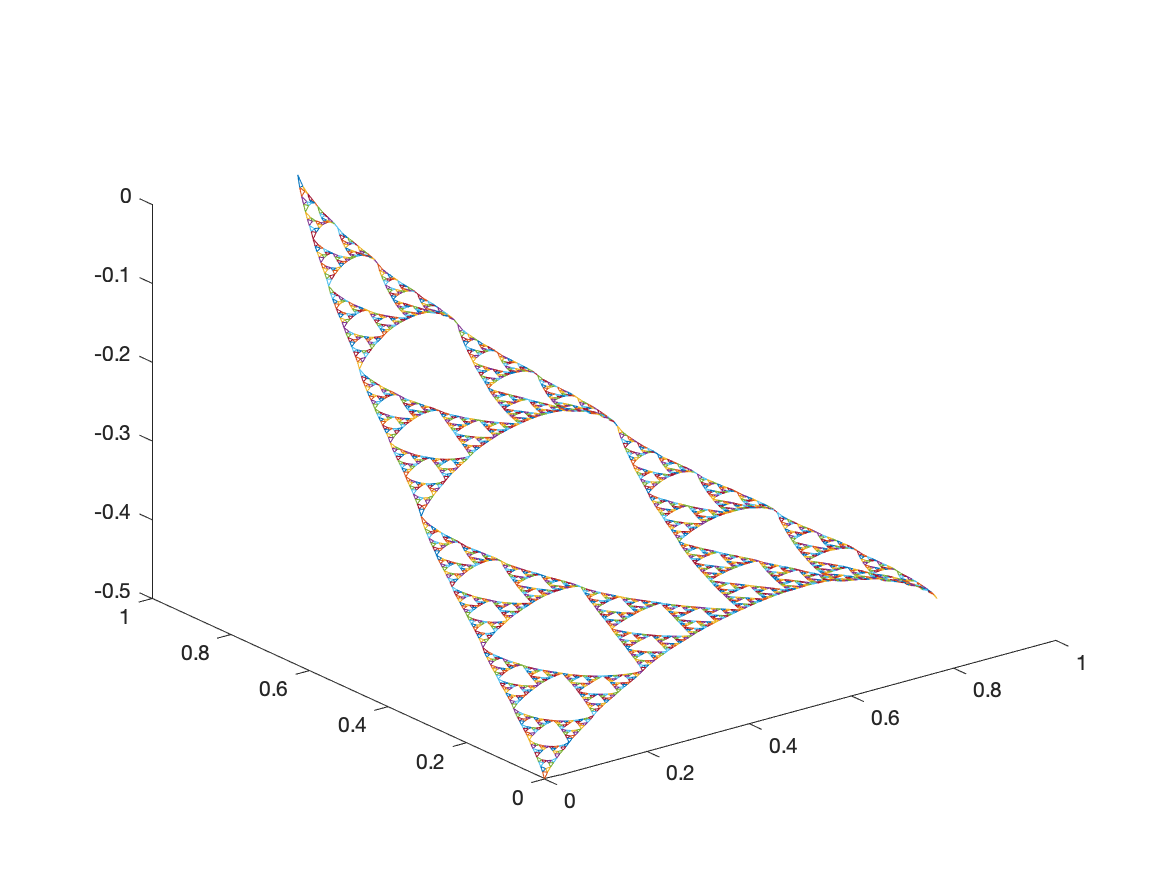
\includegraphics[width=0.75\linewidth]{Final_presentation/monomial0_2.png}
        \caption{$P_{02}$}
        
    \end{figure}
    
\end{frame}

\begin{frame}{Polynomials on SG: The monomial basis}

    \begin{figure}[H]
        \centering
        
        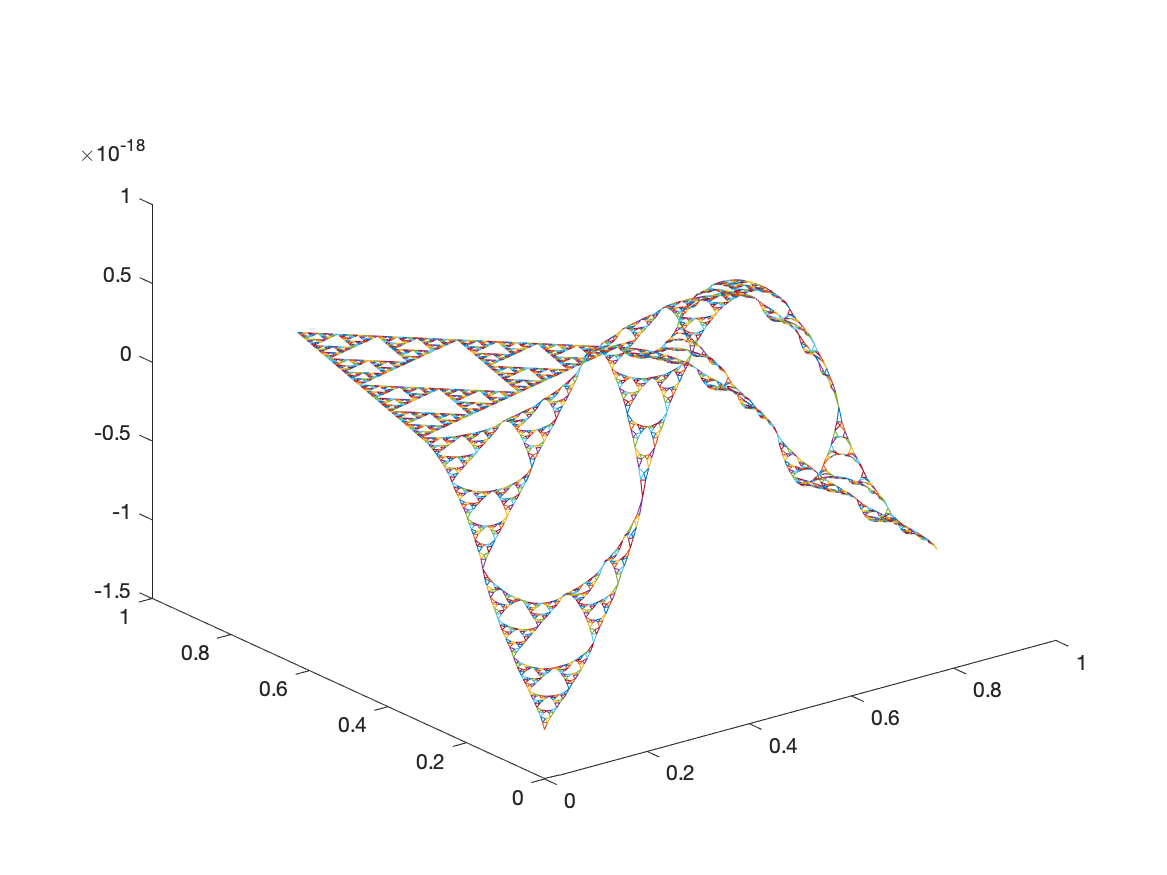
\includegraphics[width=0.75\linewidth]{Final_presentation/monomial8_2.png}
        \caption{$P_{82}$}
        
    \end{figure}
    
\end{frame}

\begin{frame}{Polynomials on SG: The monomial basis}
    \begin{figure}[H]
        \centering
        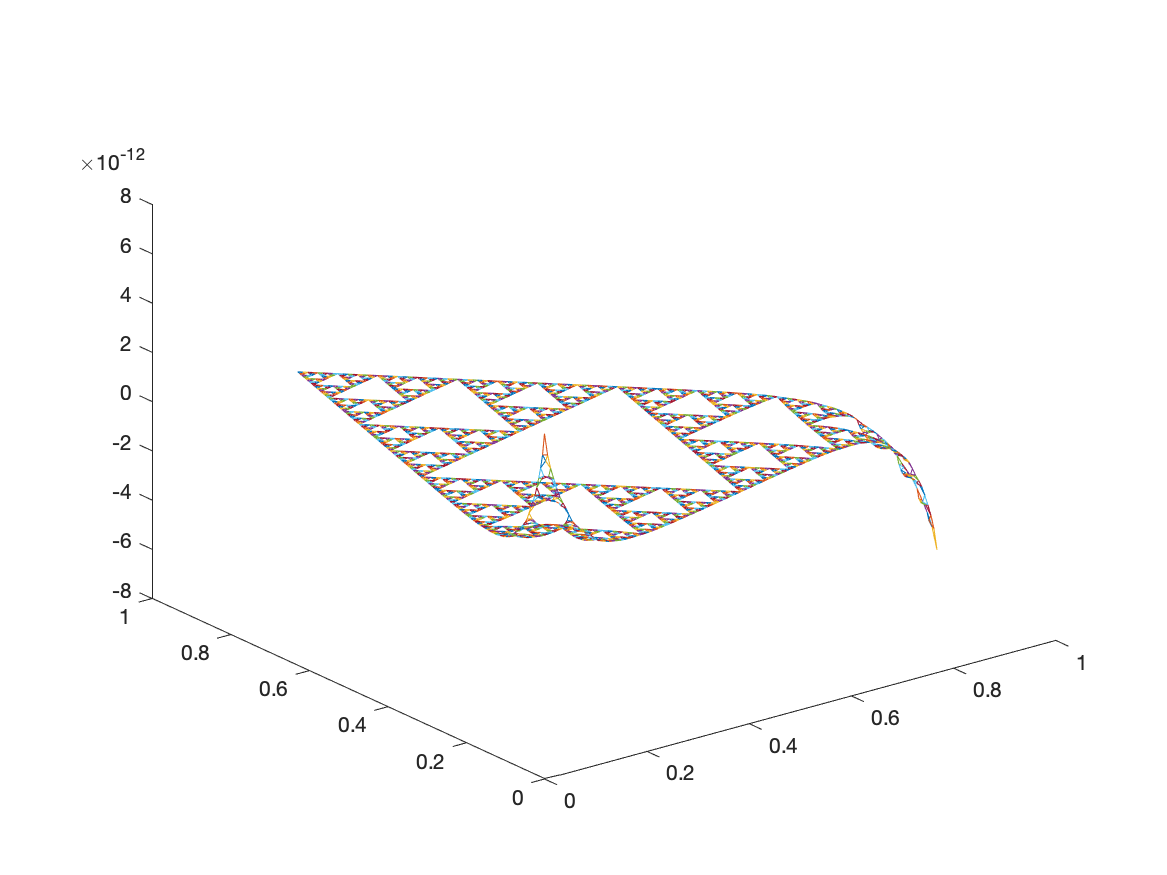
\includegraphics[width=0.75\linewidth]{Final_presentation/monomial5_3.png}
        \caption{$P_{53}$}
    \end{figure}
\end{frame}
\end{section}
\begin{section}{Sobolev Orthogonal Polynomials}
\begin{frame}{The Sobolev inner product}
    \begin{itemize}
        \item We adopt the following inner product on $\mathcal{H}_j$: 
        $$ \langle f,g \rangle_{H_1} = \int_{SG}fg + \lambda\Delta f \Delta g d\mu$$
        \item This is termed the $H^1$, or the \textbf{Sobolev inner product}.
    \end{itemize} 
    \pause
    \textbf{Question:} What are the orthogonal polynomials with respect to the Sobolev inner product? What are their properties?
\end{frame}

\begin{frame}{Main findings}
\begin{itemize}
    \item The orthogonal polynomials with respect to $k=2,3$ families satisfy a 2-term recurrence relation while those with respect to $k=1$ satisfy a 4-term recurrence: 
    $$S_{n+2} - a_nS_{n+1}-b_nS_n = f_{n+2}$$
    $$T_{n+3}-a'_nT_{n+2} - b'_nT_{n+1}-c_nT_n = f_{n+3}+d_nf_{n+2}$$
    Here $f_{n+1} = \int_{SG}G(x,y)p_{n}d\mu(y)$ where $p_{n}$ is the \textbf{nth Legendre polynomial}, the orthogonal polynomial corresponding to the $L_2$ inner product. 
\end{itemize}
\end{frame}

\begin{frame}{Main findings}
\begin{itemize}
    \item Fix $k=2,3$. Then the orthogonal polynomials corresponding to the $H^1$ inner product satisfy the following estimates: 
    
\begin{align*}
    \|\lap S_n\|_{L^2}^2&\le \lambda^{-1}\|G\|_{L^2}^2\|p_{n-1}\|_{L^2}^2+\|p_{n-1}\|_{L^2}^2 %\label{L2EstimateofSobolevLaplacian}\\
\|S_n\|_{L^{\infty}}\\
&\le C(1+\lambda^{-\frac12})\|p_{n-1}\|_{L^2} %\label{LinfinityEstimateofSobolev}\\
\|S_n(\lambda)-f_n\|_{L^2}\\
&\le 2\lambda^{-1}\|G\|_{L^2}^3\|p_{n-1}\|_{L^2}
\end{align*}

\pause
\item Moreover, $S_n(x;\lambda)$ converges to $f_n$ uniformly in $x$ as $\lambda\rightarrow\infty$. Consequently $\lap S_n\rightarrow p_{n-1}$ uniformly as $\lambda\rightarrow\infty$. Also, 
\begin{align*}
\lambda(S_n(\lambda)-f_n)\rightarrow-\frac{\langle f_n,f_{n-1}\rangle_{L^2}}{\|p_{n-2}\|_{L^2}^2}f_{n-1}-\frac{\|p_{n-1}\|_{L^2}^2}{\|p_{n-3}\|_{L^2}^2}f_{n-2} %%\label{Asymptotic extimate of S_n(lambda) to fn}
\end{align*}
uniformly in $x$ as $\lambda\rightarrow\infty$.
\end{itemize}
\end{frame}

\begin{frame}{Main findings}
    \begin{figure}
        \centering
        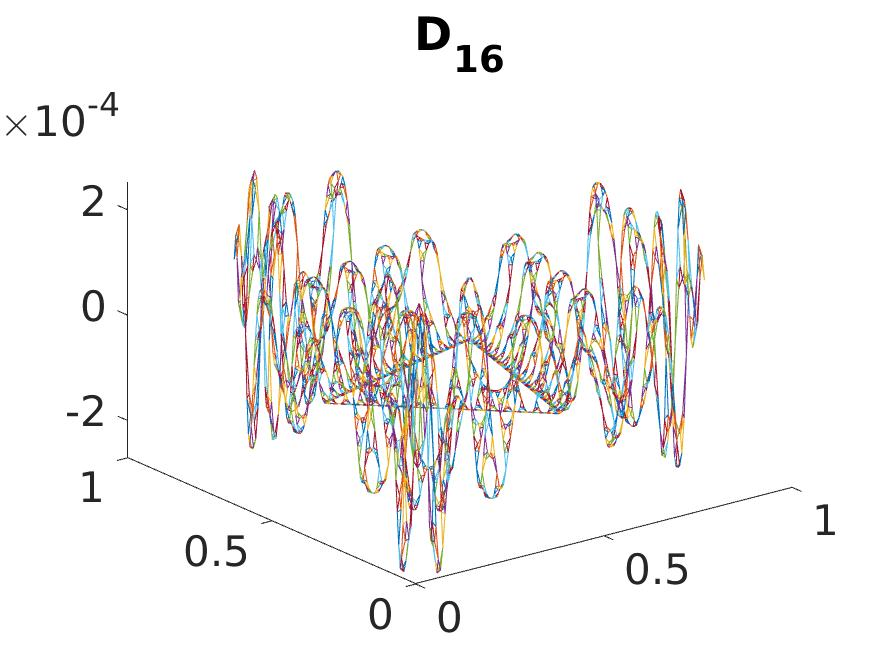
\includegraphics[width=0.5\textwidth]{images/H1SymmOPs0_19/Ss16.jpg}
        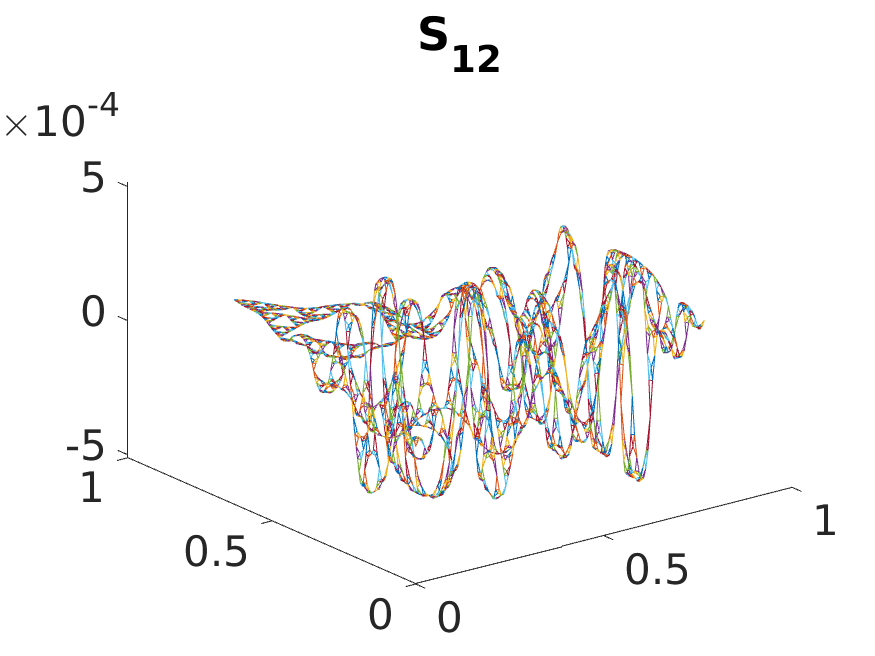
\includegraphics[width=0.5\textwidth]{images/H1AntisymOPs0_23/SAntiSym12.png}
        \caption{Sobolev orthogonal polynomials}
        %%\label{fig:my_label}
    \end{figure}
\end{frame}

\end{section}
\begin{section}{Applications and Further questions}
\begin{frame}{An Application to Interpolation and Quadrature}
    \begin{figure}
        \centering
        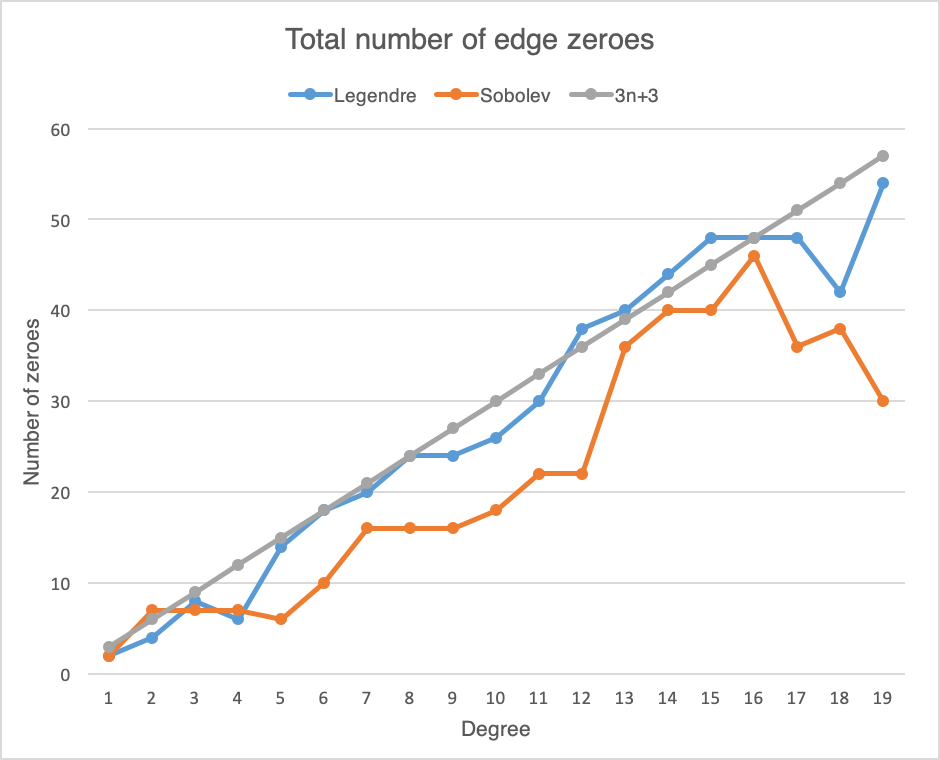
\includegraphics[width=0.7\textwidth]{images/Picture1.png}
        \caption{Edge zeroes of Anti-symmetric Sobolev and Legendre polynomials}
        %%\label{fig:my_label}
    \end{figure}
    
    Note that some $n$ degree polynomials have more than $3n+3$ zeroes! 
\end{frame}

\begin{frame}{An Application to Interpolation and Quadrature on SG}
    \begin{itemize}
        \item For which points $x_1,\ldots, x_{3n+3}$ is the matrix 
        $$M_n = \begin{bmatrix}P_{0,1}(x_1) & \ldots & P_{n,3}(x_1) \\\vdots & \ddots & \vdots \\P_{0,1}(x_{3n+3}) & \ldots & P_{n,3}(x_{3n+3})\\\end{bmatrix}$$
        invertible?
        \item Clearly not any set of $3n + 3$ points since we could take the $3n + 3$ zeroes of the polynomials found previously.
    \end{itemize}
\end{frame}

\begin{frame}{An Application to Interpolation and Quadrature on SG}
    
    \begin{itemize}
        \item On the other hand, we have the following result: For any $n\ge 0$, take $x_i=F_0^{(i-1)}(q_1)$ for $1\le i\le 2n+2$, and $x_i=F_0^{(i-2n-3)}(q_2)$ for $2n+3\le i \le 3n+3$. Then $M_n$ is invertible.
        \item We can use this information to generate a quadrature rule denoted $I_{n}^{m}$ which perfectly integrates $n$-degree polynomial splines at level $m$ with the following error bound: 
        $$\left|I_n^m(f) - \int_{SG}f\right|\leq c_1(n)5^{-(n+1)m}\|\Delta^{(n+1)}f\|_\infty$$
    \end{itemize}
\end{frame}

\begin{frame}{Further Questions}
    \begin{itemize}
        \item Characterize those sets for which $M_n$ is non-invertible.
        \item Fix $k=1$. Prove that for every $n \geq 0$, $\partial_nf_{n}(q_0) \neq 0$.
    \end{itemize}
\end{frame}
\end{section}

% The theory of Sobolev orthogonal polynomials on $\mathbb{R}$ is well known and has gathered interest over the last 20 years. We build on this body of work by defining a Sobolev inner product on the Sierpinski Gasket and studying the corresponding Sobolev orthogonal polynomials. We find recurrence relations in the sequences of these polynomials and study their finer properties such as their $L^2$, $L^\infty$ and $H^1$ norms. We also use the Sobolev orthogonal polynomials to further understand the question around polynomial interpolation. Finally, we study the analogues of the Chebyshev polynomials and present some preliminary results and background related to them. 
\end{document}
